\section*{APPENDIX B - Datasets and Code}
\addcontentsline{toc}{section}{APPENDIX B - Datasets and Code}
%\addcontentsline{toc}{section}{APPENDIX B - Thesis Planning}
%Time should be allocated to thesis writing and review as well as technical progress.
%A Gantt chart displaying the expected progress over the course of the two semesters
%is shown in \cref{fig:gantt_chart}. Note that a significant portion of time at the beginning was allocated
%to initial research and project scope. Due to the large number of students working on this team,
%a clear project scope was important so that students did not unnecessarily duplicate work.

%\begin{figure}[H]
%    \centering
%    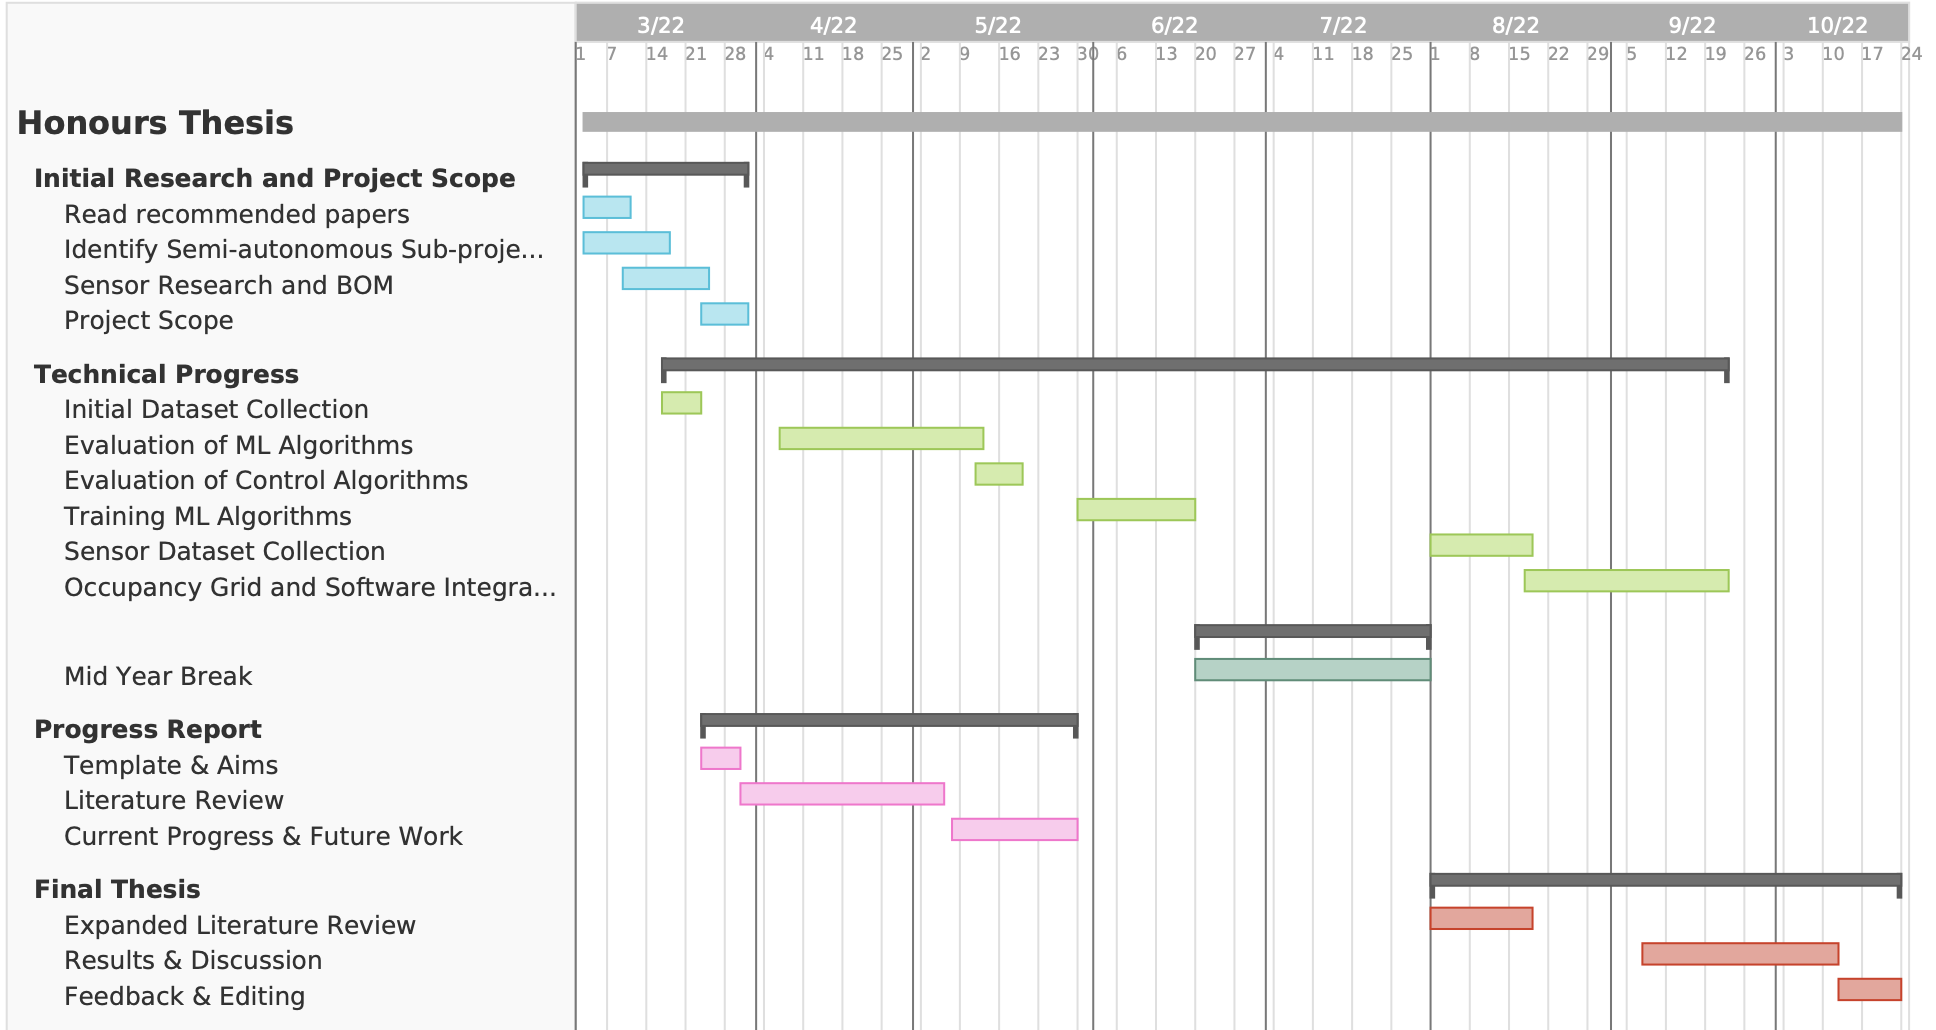
\includegraphics[width=\linewidth]{images/gantt_chart.png}
%    \caption{Gantt chart of thesis progress}
%    \label{fig:gantt_chart}
%\end{figure}
% TODO update Gantt chart

Code: \href{https://github.com/JakobWyatt/smart-wheelchair}{\underline{Github}}.
ZED Dataset: \href{https://curtin.sharepoint.com/:f:/r/sites/CurtinXGlide/Shared%20Documents/Navigation%20and%20Object%20Detection/ZED?csf=1&web=1&e=tTau9D}{\underline{Curtin X Glide (Smart Wheelchair)}} Teams channel.
Preliminary Dataset: \href{https://curtin.sharepoint.com/:v:/r/sites/CurtinXGlide/Shared%20Documents/Navigation%20and%20Object%20Detection/GoPro%20Dataset.mp4?csf=1&web=1&e=seLdRb}{\underline{(also hosted on teams)}}.
